\documentclass{ltjsarticle}

\usepackage{amsmath}
\usepackage{amssymb}
\usepackage{amsthm}
\usepackage{ mathrsfs }
\usepackage{enumerate}
\usepackage{bbm}
\usepackage{lipsum}
\usepackage{fancyhdr}
\usepackage{tikz-cd} 
\usetikzlibrary{graphs}
\usepackage{luatexja-ruby} 
\usepackage{graphicx} 
\graphicspath{ {./../../images/} }

\newtheorem{theorem}{定理}[section] 
\newtheorem{proposition}{Proposition}[section] 
\newtheorem{definition}{定義}[section] 
\newtheorem{problem}{問題}
\newtheorem{postulate}{公準}[section] 
\newtheorem{lemma}{Lemma}[section] 
\newtheorem{notation}{Notation}[section] 
\newtheorem{remark}{注釈}[section] 
\newtheorem{corollary}{系}[section] 
\newtheorem{terminology}{Terminology}[section] 
\newtheorem{example}{例}[section] 
\newtheorem{step}{手順} 
\newtheorem{solution}{解答}[section] 
\newtheorem{fact}{事実}[section] 


\DeclareMathOperator{\diam}{diam}
\DeclareMathOperator{\Gal}{Gal}
\DeclareMathOperator{\rank}{rank}
\DeclareMathOperator{\Hom}{Hom}
\DeclareMathOperator{\Dom}{Dom}
\DeclareMathOperator{\Ann}{Ann}
\DeclareMathOperator{\grad}{grad}
\DeclareMathOperator{\Span}{Span}
\DeclareMathOperator{\interior}{int}
\DeclareMathOperator{\ind}{ind}
\DeclareMathOperator{\supp}{supp}
\DeclareMathOperator{\ob}{ob}
\DeclareMathOperator{\Spec}{Spec}
\DeclareMathOperator{\MaxSpec}{MaxSpec}
\DeclareMathOperator{\PreSh}{PreSh}
\DeclareMathOperator{\Sh}{Sh}
\DeclareMathOperator{\Fun}{Fun}
\DeclareMathOperator{\Ext}{Ext}
\DeclareMathOperator{\Aut}{Aut}
\DeclareMathOperator{\Ker}{Ker}
\DeclareMathOperator{\Image}{Im}
\DeclareMathOperator{\Coker}{Coker}
\DeclareMathOperator{\id}{id}
\DeclareMathOperator{\Mod}{Mod}
\DeclareMathOperator{\QCoh}{QCoh}
\DeclareMathOperator{\Coh}{Coh}
%\newcommand*{\name}[\num_arguments][default values]{{\color{#1}\Large #2}}
\newcommand*{\Z}{\mathbb{Z}}
\newcommand*{\Q}{\mathbb{Q}}
\newcommand*{\R}{\mathbb{R}}
\newcommand*{\multivar}[2]{{#1_1,\cdots,#1_{#2}}}
\newcommand*{\localization}[2]{#1_{\mathfrak{#2}}}
\newcommand*{\ringedspacemorph}[1]{(#1,#1^{\#})}
\newcommand*{\sheaf}[2]{(#1,{\mathcal{#2}}_{#1})}
\newcommand{\fib}[1]{%
  \mathbin{\mathop{\times}\limits_{#1}}%
}
\newcommand{\tens}[1]{%
  \mathbin{\mathop{\otimes}\displaylimits_{#1}}%
}
\title{授業ノート}
\author{ボン補習校高校数学}
\date{５月９日}

\begin{document}

\maketitle
微分を今まで${\frac d {dx}}f$と書いてきましたが、長いので$f'(x)$と書くようにします。最初のはオランダ人数学者ライプニッツが作った記号で$f'(x)$はフランス人数学者ラグランジュが作りました。
\section{商の微分}

\begin{theorem}
$\lim_{n\to\infty}a_n\alpha,\lim_{n\to\infty}b_n=\beta$となるような数$\alpha,\beta$が存在するなら
\begin{equation*}
\lim_{n\to \infty}a_nb_n = \lim_{n\to\infty}a_n\lim_{n\to\infty} b_n
\end{equation*}
\end{theorem}
要するに極限が存在する時、掛け算と極限を取る$\lim_{n\to\infty}$は交換することができるということを言っています。また
\begin{theorem}
$f(x)$が$a$で連続で$f(a)\not=0$ なら${\frac 1 {f(x)}}$も$a$で連続。つまり、
\begin{equation*}
\lim_{x\to a}{\frac 1 {f(x)}} = {\frac 1 {f(a)}}
\end{equation*}
\end{theorem}
\begin{theorem}
$\lim_{h\to0}{\frac {f(x+h)-f(x)} h}$が存在して$f(x)\not=0$なら、
\begin{equation*}
\left({\frac 1 {f(x)}}\right)' =- {\frac {f'(x)} {(f(x))^2}}.
\end{equation*}
\end{theorem}
\begin{proof}[証明]
\begin{align*}
f'(x) = \lim_{h\to0}{\frac {f(x+h)-f(x)} h}
\end{align*}
を思い出しましょう。
\begin{equation*}
\left({\frac 1 {f(x)}} \right)'= \lim_{h\to\infty}{\frac {{\frac 1 {f(x+h)}}-{\frac 1 {f(x)}}} {h}}
\end{equation*}
なので分子を先に計算してみやすくしてみましょう。
\begin{equation*}
{\frac 1 {f(x+h)}}-{\frac 1 {f(x)}} \stackrel{\text{通分して}}{=}\underbrace{\underline{\quad\quad\quad}}_{\text{自分で計算してみよう}}
\end{equation*}
計算した結果を元の式に入れて、
\begin{equation*}
\lim_{h\to 0}{\frac {\quad\quad\quad\quad} h} = \lim_{h\to0}{\frac 1 {f(x+h)f(x)}}\lim_{h\to 0}{\frac {f(x)-f(x+h)} h}
\end{equation*}
ここで${\frac 1 {f(x)}}$は連続なので$h=0$をそのまま代入できる。
\begin{equation*}
\lim_{h\to 0}{\frac {f(x)-f(x+h)} h} =- \lim_{h\to 0}{\frac {f(x+h)-f(x)} h} = -f'(x).
\end{equation*}
よって最初の定理を使うと証明ができる。
\end{proof}
ここで、
\begin{equation*}
f(x) = \sum_{k=0}^\infty {\frac 1 {k!}}x^k
\end{equation*}
とする。上の定理を${\frac {f(x)} {e^x}}$に使うことを考える。$f'(x) = f(x)$となることを思い出そう。まず$e^x>0$なので定理が使えるまた、次の定理と組み合わせてみる。
\begin{equation*}
(fg)'(x) = g(x)f'(x)+f(x)g'(x).
\end{equation*}
すると、次の定理を得る。
\begin{theorem}
\begin{equation*}
\left({\frac {g(x)}{f(x)}}\right)' = {\frac {f(x)g'(x)-g(x)f'(x)} {f(x)^2}}
\end{equation*}
\end{theorem}

\begin{proof}[証明]
\begin{align*}
(fg)'(x)& = g(x)\left({\frac 1 {f(x)}}\right)'+{\frac 1 {f(x)}}g'(x),\\
& = -{\frac {g(x)f'(x)} {f(x)^2}}+{\frac {g'(x)} {f(x)}}
\end{align*}
通分して
\begin{equation*}
=\underbrace{\quad\quad\quad\quad\quad}_{\text{自分で証明してみよう}}
\end{equation*}
\end{proof}

\begin{equation*}
\left({\frac {f(x)} {e^x}}\right)' = {\frac {f'(x)e^x-f(x)e^x } {e^{2x}}}= {\frac {f(x)e^x-f(x)e^x} {e^{2x}}}=0
\end{equation*}
つまり${\frac {f(x)} {e^x}}$は変化をしない。ということは${\frac {f(x)} {e^x}}$は常に一定、つまり定数。さらに言い換えると、
\begin{equation*}
{\frac {f(x)} {e^x}} = {\frac {f(0)} {e^0}} = f(0) = 1
\end{equation*}
となるので、両辺に$e^x$を掛けると
\begin{equation*}
f(x) = e^x
\end{equation*}
となります。
\begin{remark}
\begin{equation*}
f(x) = 1+x+{\frac 1 {2!}}x^2 +\cdots
\end{equation*}
という形を使ったのは最後の$f(0) = 1$となるところだけでした。それ以外では
\begin{equation*}
f'(x) = f(x)
\end{equation*}
という性質しか使っていません。つまりこの計算が示すことは、ある物体または対象の最初の状態とそのあとどのように変化するのかがわかっていれば全ての時間において物体の動きや対象の変化を正確に知ることができるということです。
\end{remark}
\section{テイラー展開}
\begin{equation*}
y = f'(a)(x-a)+f(a)
\end{equation*}
これを$f(x) = (x-1)^2$、$a=2$の時に考える。
\begin{theorem}
ある点$(x_0,y_0)$を通って傾きが$a$の直線の公式は
\begin{equation*}
y-y_0 = a(x-x_0)
\end{equation*}
となる。
\end{theorem}
\begin{proof}[証明]
もし平面上の点$(x,y)$が直線の上にあれば傾きが$a$なので
\begin{equation*}
{\frac {(y-y_0)} {(x-x_0)}} = a
\end{equation*}
となるため。
\end{proof}
傾きを計算すると
\begin{equation*}
f'(x) = \underbrace{\underline{\quad\quad\quad}}_{\text{自分で計算してみよう}}
\end{equation*}
なので
$f(2) = 1,f'(2) = 2$となります。ここで次の直線を考えます
\begin{equation*}
y -1 = 2(x-2)
\end{equation*}

両辺に$1$を足して、展開して
\begin{equation*}
y = 2x-3
\end{equation*}
となります。これは元のグラフをどのくらい正確に捉えているでしょうか。もちろん$x=2$での値が一緒になります、それ以外の場所では二つのグラフの差は
\begin{equation*}
f(x) - 2x+3 = x^2-2x+1 - 2x +3 = x^2-4x+4 = (x-2)^2
\end{equation*}
となります。$2$乗の形になったのは偶然でしょうか。この数式が示す意味を次回の授業で取り扱います。
\section{問題}
\par\textbf{微分}
\par\textbf{問題：}次の関数の微分を計算せよ。
\begin{equation*}
3x^2+x+1,x^3+3x^2+3x+1,3e^x+5x
\end{equation*}

\textbf{問題：}$e^x$の$x=0$での接線を求めて、元のグラフとの差が
\begin{equation*}
{\frac {x^2} {2!}}+{\frac {x^3} {3!}}+\cdots
\end{equation*}
になることを確認しよう。
\par \textbf{チャレンジ課題：変数変換}
\par 二つの微分可能な関数$f,u$について$(f\circ u)(x) = f(u(x))$とします。例えば$f(x) = x^2, u=x+1$なら$(f\circ u)(x) = (x+1)^2$となります。ここで$f\circ u$の微分を考えてみましょう。
\begin{equation*}
\lim_{h\to 0}{\frac {f(u(x+h))-f(u(x))} {h}} \stackrel{1={\frac {u(x+h)-u(x)} {u(x+h) -u(x)}}\text{を掛けて}}{=} \lim_{h\to 0}{\frac {u(x+h)-u(x)} {h}}\cdot\lim_{h\to 0}{\frac {f(u(x+h))-f(u(x))} {u(x+h)-u(x)}}
\end{equation*}
ここで極限の定義を思い出しましょう。
\begin{equation*}
\lim_{x\to a}g(x)= \alpha
\end{equation*}
になると言うのはどんな数列$(a_n)_{n=1,2,\cdots}$でももし
\begin{equation*}
\lim_{n\to\infty}a_n = a
\end{equation*}
となるなら、
\begin{equation*}
\lim_{n\to \infty}g(a_n) = \alpha
\end{equation*}
となることでした。ここで$u(x)$は連続なので
\begin{equation*}
\lim_{h\to0}u(x+h) = u(x)
\end{equation*}
となります。なので
\begin{equation*}
\lim_{h\to 0}(u(x+h)-u(x)) = 0
\end{equation*}
ここで$a_n = u\left(x+{\frac 1 n}\right)-u(x)$とおくと$\lim_{n\to\infty}a_n = 0$これを使って
\begin{equation*}
 \lim_{h\to 0}{\frac {f(u(x+h))-f(u(x))} {u(x+h)-u(x)}} =  \lim_{n\to \infty}{\frac {f(u(x)+a_n)-f(u(x))} {a_n}}=\lim_{h\to 0}{\frac {f(u(x)+h)-f(u(x))} {h}} = f'(u(x))
\end{equation*}
となります。$\lim_{h\to 0}{\frac {u(x+h)-u(x)} {h}} = u'(x)$なので掛け算すると
\begin{equation*}
(f\circ u)'(x)= \lim_{h\to 0}{\frac {f(u(x+h))-f(u(x))} {h}} = \lim_{h\to 0}{\frac {u(x+h)-u(x)} {h}}\cdot{\frac {f(u(x+h))-f(u(x))} {u(x+h)-u(x)}} = u'(x)f'(u(x))
\end{equation*}
となります。
\par\textbf{例：}$(x+1)^2$の微分を$f(x) = x^2,u(x) = x+1$とすると$f\circ u(x) = (x+1)^2$なるまた$f'(x) = 2x,u'(x) = 1$よって
\begin{equation*}
((x+1)^2)' = (f\circ u)'(x) = 1\cdot 2(x+1)
\end{equation*}
\par\textbf{チャレンジ問題：}次の関数の微分をしてみよう。
\begin{equation*}
(x+1)^3,(2x+1)^2(x^2+2)^4
\end{equation*}
\par\textbf{グラフ理論：オイラーグラフ}\\
\textbf{問題：}次のグラフを一筆で書くことを考える。
\begin{center}
\begin{figure}[h]
	\centering
    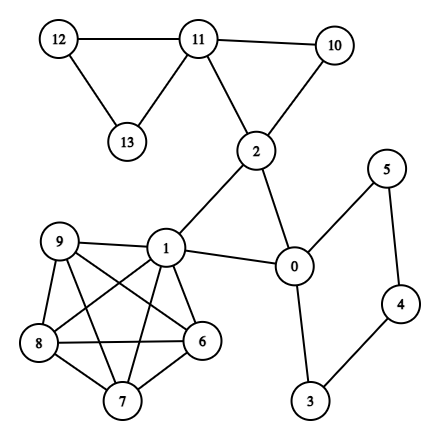
\includegraphics[scale=0.25]{euler_graph_big}
    \label{fig:Euler_1}
\end{figure}
\end{center}
\begin{center}
最初のグラフからまんなかの$0-1-2$のサイクルを取り除いたグラフ
\begin{figure}[h]
	\centering
    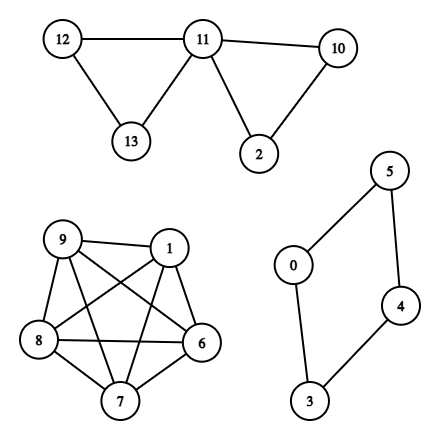
\includegraphics[scale=0.25]{euler_graph_disconnected}
    \label{fig:Euler_1}
\end{figure}
\end{center}
三つのグラフに分かれました。それぞれ一筆書きできますか？これをつかって元のグラフを一筆書きすることを考えてみましょう。
\par\textbf{チャレンジ問題：}もし元のグラフが一筆で書けるなら、そこからサイクルを取り除いたグラフは一筆書きできるいくつかのグラフに分かれます。これはなぜでしょうか。（サイクルの辺を取り除いた時繋がれていた頂点はそれぞれいくつ次数が減ったかな？）
\par\textbf{整数論：合同式}

$n$を整数とする時、二つの整数$a,b$が$n$を法として合同とは$b-a$が$n$で割れる時、言い換えて$a,b$の$n$で割った時の余りが同じことを言います。これを
\begin{equation*}
a\equiv b\mod{n}
\end{equation*}
と書きます。これを使うと全ての整数を$n$で割った余りで分類することができます。
\par\textbf{問題：}$n=2,3,7,11$の時それぞれ可能な余りはいくつですか。例えば$n=5$のとき可能な余りは$0,1,2,3,4$です。
\par\textbf{問題：}次の二つを証明してみましょう。もし$a\equiv b\mod{n},c\equiv d\mod{n}$ならば
\begin{enumerate}
\item $a+b\equiv c+d\mod{n}$
\item $ac \equiv bd\mod{n}$
\end{enumerate}

\par\textbf{ステップ１：}示したいのは
\begin{equation*}
(c+d)-(a+b)
\end{equation*}
が$n$で割れること。私たちが知っているのは
\begin{equation*}
(b-a),(d-c)
\end{equation*}
が$n$で割れること（二つは$n$の約数）。これを使って$(c+d)-(a+b)$を$n$の約数の和にできないだろうか。
\par\textbf{ステップ２：}最初と同じように$bd-ac$が$n$で割れることを知りたい。
$bc-bc = 0$なので
\begin{equation*}
bd-ac = bd-ac+0 = bd-ac -bc+bc
\end{equation*}
最後の形をうまく変形して$n$の倍数の和にしよう。
\par\textbf{問題：}$2^{100}$と$3^{100}$の一の位の数を調べてみよう。ここで、
\begin{equation*}
2^1 \equiv 2 \mod{10},2^2 \equiv 4 \mod{10},2^3 \equiv 8 \mod{10},2^4 \equiv 6 \mod{10},2^5 \equiv 2 \mod{10},
\end{equation*}
になることに注意しよう。指数法則をつかうと$(2^a)^b = 2^{ab}$となります。最初の問題で見たように、余りの式では掛け算が使えます。なので指数法則はあまりの式でも使えます。例えば上の式で$2^5\equiv 2\mod{10}$なので、
\begin{equation*}
2^{10} \equiv (2^5)^2 \equiv 2^2 \equiv 4 \mod{10}
\end{equation*}
つまり$2^{10}$の一の位は$4$。これを使って$2^{100},3^{100}$の一の位の数を調べてみよう。
\par\textbf{図形：三角形の外心と内心}\\
\textbf{問題：}$OD,OE$はそれぞれ辺$AB,BC$を垂直に半分にする線。ここで$OA=OB=OC$となることを確かめよう。また$F$がちょうど辺$CA$の真ん中の時$OF$が$CA$に垂直になること示そう。（ヒント：この問題は$\triangle OAB,\triangle OBC$がそれぞれ二等辺三角形になることを聞いています。そのことを証明するためにどのような合同な三角形を見つければ良いでしょうか。）
\begin{center}
\begin{figure}[h]
	\centering
    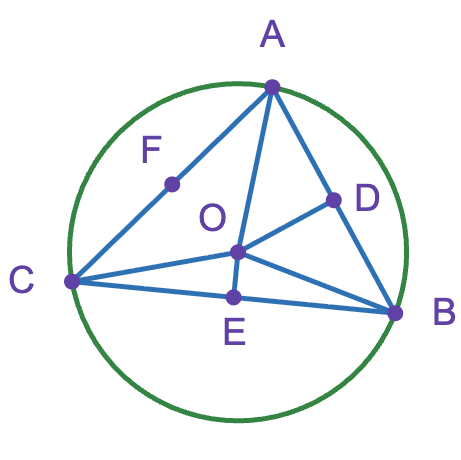
\includegraphics[scale=0.25]{outer_center}
    \label{fig:Euler_1}
\end{figure}
\end{center}
\textbf{問題：}$OA,OB$は角$A,B$をそれぞれ半分にする線です。ここで$OI,OG$をそれぞれ$AB,BC$に垂直な線とすると$OI=OG$となることを示そう。また$CA$上の点$H$を$OH$が$CA$に垂直になるように引くと、$OH=OI=OG$になることと$OC$が角$C$を半分にすることも示そう。（ヒント：外心の時と同じように合同な三角形を見つけてみよう。最後の部分はピタゴラスの定理を使うと簡単になります。）
\begin{center}
\begin{figure}[h]
	\centering
    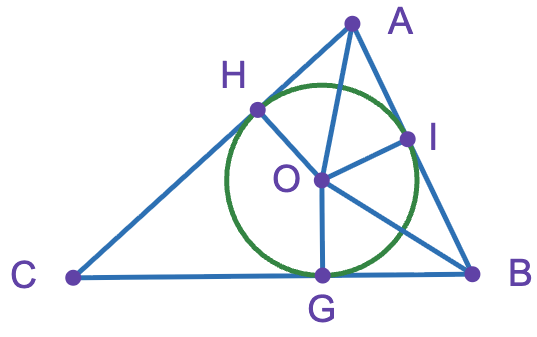
\includegraphics[scale=0.25]{inner_center}
    \label{fig:Euler_1}
\end{figure}
\end{center}

\end{document}